\documentclass[11pt,a4paper]{article}

\usepackage[utf8]{inputenc}
\usepackage{amsmath,amssymb}
\usepackage{graphicx}
\usepackage{hyperref}
\usepackage{geometry}
\usepackage{caption}
\geometry{margin=1in}

\title{Differentially Private Federated Learning (DP-FL) on CIFAR-10}
\author{Rudra}
\date{October 2026}

\begin{document}

\maketitle

\begin{abstract}
This project implements and evaluates a Differentially Private Federated Learning (DP-FL) system on the CIFAR-10 dataset. By combining Flower for federated orchestration and Opacus for Differential Privacy (DP), we investigate the privacy-utility tradeoff under realistic non-IID data distributions (Dirichlet $\alpha=0.1$). Our comprehensive evaluation across varying noise multipliers ($\sigma$), clipping thresholds ($C$), and data heterogeneity levels demonstrates that DP protects individual data samples at the cost of model utility. The negative impact on convergence appears empirically associated with high data heterogeneity under the tested configurations.
\end{abstract}

\section{Introduction}

Federated Learning (FL) allows distributed edge devices to collaboratively train a shared model without transmitting raw data to a central server. However, exchanging model weights or gradients remains vulnerable to inference attacks, where adversaries can reconstruct original training examples. Differential Privacy (DP) mitigates this by injecting calibrated noise and clipping gradients, providing a mathematical guarantee of privacy. In this work, we train a CNN on CIFAR-10 distributed across 5 clients, exploring how data heterogeneity interacts with DP-SGD mechanisms.

\section{Problem Statement}

The objective is to train a convolutional neural network on a heavily skewed, non-IID partition of CIFAR-10 across distributed clients. The system must provide an $(\varepsilon,\delta)$-differential privacy guarantee for individual training samples, with the global guarantee obtained under the stated parallel-composition assumption across disjoint client datasets. We aim to quantify how much accuracy is sacrificed for strong privacy guarantees, particularly when the underlying local data is highly specialized (non-IID).

\section{Background}

\subsection{Federated Learning}

FL operates through synchronized rounds. The server broadcasts a global model, clients train locally, and the server aggregates the updates (e.g., via FedAvg).

\subsection{Differential Privacy \& DP-SGD}

DP guarantees that a single data sample's presence or absence does not statistically alter the algorithm's output probability beyond a bound $e^\varepsilon$. DP-SGD achieves this by computing per-sample gradients, clipping them to a maximum $L_2$ norm $C$, and adding Gaussian noise scaled by $C$ and $\sigma$.

\subsection{Rényi Differential Privacy (RDP)}

RDP tracks the privacy loss analytically across multiple training steps using Rényi divergence. RDP provides tighter composition bounds for Gaussian mechanisms compared to standard DP, allowing us to safely convert the cumulative RDP back to $(\varepsilon, \delta)$ metrics after training.

\section{Threat and Privacy Motivation}

A malicious server or a compromised client intercepting updates could execute membership inference or data reconstruction attacks. Our threat model assumes an honest-but-curious server and adversarial participants. DP protects against these threats by ensuring that any output weight matrix is statistically indistinguishable regardless of any single participant's specific training samples.

\section{Methodology}

Our methodology proceeds in sequential stages:

1. Dirichlet data partitioning to simulate non-IID data.

2. Centralized training baseline.

3. Standard Federated Learning (FedAvg).

4. Differentially Private Federated Learning (DP-FedAvg).

5. Grid search over DP hyperparameters ($C, \sigma$).

6. Ablation over data heterogeneity ($\alpha, \sigma$).

\section{System Architecture}

We use the \textbf{Flower} (\texttt{flwr}) framework to orchestrate virtual clients. Instead of physical network distribution, we leverage the \textbf{Ray} Virtual Client Engine to simulate massive concurrency on a single machine or GPU. The local training loop uses standard PyTorch, wrapped entirely by \textbf{Opacus}.

\section{Dataset and Non-IID Partitioning}

The CIFAR-10 dataset (50k train, 10k test) is partitioned across 5 clients using a Dirichlet distribution.

\begin{itemize}
    \item \textbf{$\alpha=0.1$}: High heterogeneity (official setup). Clients typically hold only 1-2 classes dominantly.
    \item \textbf{$\alpha=10.0$}: Low heterogeneity (near-IID). Clients have an approximately uniform mix of all 10 classes.
\end{itemize}

\begin{figure}[h]
    \centering
    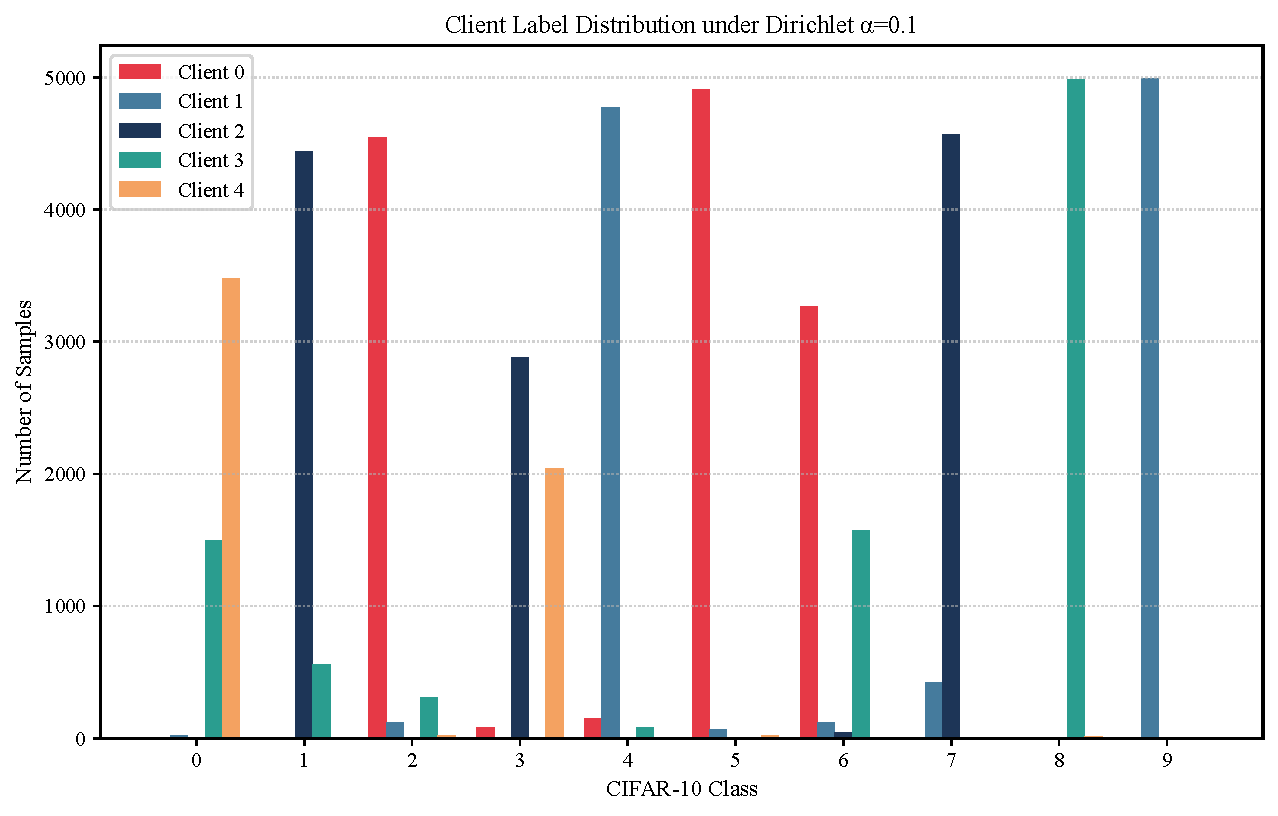
\includegraphics[width=0.8\textwidth]{figures/fig1_stage1_distribution.pdf}
    \caption*{Client Label Distribution under Dirichlet $\alpha=0.1$. Note how clients receive disjoint class concentrations.}
    \label{fig:stage1}
\end{figure}

\section{Model Architecture}

We use a SimpleCNN designed explicitly for DP:

\begin{itemize}
    \item 3 Convolutional layers ($3\to16\to32\to64$ channels)
    \item \textbf{GroupNorm} instead of BatchNorm (crucial, as BatchNorm breaks per-sample independence)
    \item MaxPool \& ReLU activations
    \item Fully Connected layer ($64\times4\times4 \to 128 \to 10$)
    \item Dropout ($p=0.5$) for regularization
\end{itemize}

\section{Federated Training Procedure}

\begin{itemize}
    \item \textbf{Clients}: 5
    \item \textbf{Rounds}: 3
    \item \textbf{Local Epochs}: 1
    \item \textbf{Batch Size}: 64
    \item \textbf{Optimizer}: SGD, Learning Rate: 0.05
    \item \textbf{Aggregation}: FedAvg
\end{itemize}

\section{DP Mechanism}

We implement DP using Opacus. The \texttt{PrivacyEngine} wraps the local model, optimizer, and dataloader. The dataloader uses Poisson sampling to create batches, computing true per-sample gradients.

\begin{itemize}
    \item \textbf{Clipping}: Per-sample gradient $L_2$ norms are bounded to $C \in \{0.1, 1.0\}$.
    \item \textbf{Noise}: Gaussian noise scaled by $\sigma \in \{0.5, 1.0, 1.5, 2.0\}$ is added to the batch-averaged gradient.
\end{itemize}

\section{Privacy Accounting}

We utilize Rényi Differential Privacy (RDP) to track the privacy loss analytically. Because the dataset is statically partitioned using a Dirichlet distribution and clients hold disjoint datasets, we leverage \textbf{parallel composition} across clients. The global privacy guarantee is bounded by the privacy loss of the worst-case individual client. The complete accounting chain is derived as follows.

We explicitly define the parameters of the privacy accountant:
\begin{itemize}
    \item $\alpha$: Rényi order (distinct from the Dirichlet data heterogeneity parameter).
    \item $\delta$: The target global failure probability, fixed to $10^{-5}$.
    \item $\sigma$: The noise multiplier.
    \item $C$: The per-sample gradient clipping norm.
    \item $q$: The sampling rate (expected batch size divided by local dataset size).
    \item $T$: The total number of physical DP steps performed by a client.
\end{itemize}

\subsection{Per-Step Subsampled Gaussian Mechanism}

At each training step, the dataloader draws a batch with sampling rate $q$. Opacus computes the per-sample gradients and clips them to a maximum $L_2$ norm $C$. It then adds Gaussian noise with standard deviation $\sigma C$ to the batch-averaged gradient. Note that while $C$ determines the absolute sensitivity and noise scale added to the gradients, it does not appear directly in the privacy accountant's $\varepsilon$ calculation because the $\sigma$ provided to Opacus already defines the noise multiplier relative to the sensitivity (i.e., noise standard deviation is $\sigma C$, so the ratio of noise to sensitivity is simply $\sigma$).

\subsection{Rényi Differential Privacy (RDP) Composition}

For a single DP-SGD step, the privacy loss is quantified by the RDP of order $\alpha$, denoted as $\text{RDP}_{\text{step}}(\alpha, q, \sigma)$. Because we assume sequential composition over the DP steps performed by a single client, for $T$ total local steps, the accumulated RDP is:

\begin{equation}
    \text{RDP}_T(\alpha) = T \cdot \text{RDP}_{\text{step}}(\alpha, q, \sigma)
\end{equation}

\subsection{Conversion to $(\varepsilon, \delta)$-DP}

The cumulative RDP is converted back to standard $(\varepsilon, \delta)$-DP. We use the exact conversion formula implemented by the Opacus accountant, which is based on the optimal conversion theorem \cite{balle2020}:

\begin{equation}
    \varepsilon_\alpha(\delta) = \text{RDP}_T(\alpha) - \frac{\log \delta + \log \alpha}{\alpha - 1} + \log\left(\frac{\alpha - 1}{\alpha}\right)
\end{equation}

The reported $\varepsilon$ for the client is the minimum over all evaluated Rényi orders $\alpha$:

\begin{equation}
    \varepsilon = \min_\alpha \varepsilon_\alpha(\delta)
\end{equation}

Finally, under the parallel composition assumption for disjoint client datasets, the global reported epsilon is simply $\max(\varepsilon_{\text{clients}})$.

\subsection{Experimental Application}

In our experiments, we fix $\delta = 10^{-5}$. The RDP accountant uses the actual sample rate $q$ extracted from the \texttt{DPDataLoader} and the exact accumulated DP step count $T$ for each client. The parameters $\sigma$ and $C$ are defined by the specific experimental run, and the final $\varepsilon$ (with its corresponding minimizing Rényi order) is recorded directly from the Opacus accountant in the run artifacts.

\textbf{Concrete Example (Stage 4)}:

In the authoritative 15-round Stage 4 run ($\sigma=1.0, C=1.0$), a client performed $T = 3045$ total DP steps. Evaluated at $\delta = 10^{-5}$, the Opacus accountant identified a minimizing Rényi order of $r = 6.9$, yielding a final worst-case global privacy guarantee of $\varepsilon = 2.6974$.

\section{Experimental Setup}

Experiments were initially intended to run on a GPU environment (Tesla T4 via Colab) to overcome Ray compatibility issues on Windows and accelerate Opacus's computationally expensive per-sample gradient hooks. However, empirical analysis of the generated execution artifacts (e.g., `results/stage4/summary.json`) confirms that the authoritative 15-round Stage 4 run, as well as the Stage 2 and Stage 3 baselines, actually executed on a CPU device (`"device": "cpu", "GPU": "None"`). Consequently, the substantial recorded runtimes (such as Stage 4's ~1784.72 seconds, which conflicts with an outer-wrapper `runtime.json` timestamp of ~721.84 seconds, likely due to nested timing scopes) reflect CPU-bound performance. Stage 5 full grid results, by contrast, indicate they successfully leveraged CUDA (`"device": "cuda"`). We report the actual execution hardware as recorded in the provenance artifacts rather than the planned configuration.

\section{Results}

\subsection{Centralized Baseline (Stage 2)}

Training the model centralized on the full 50,000 CIFAR-10 images for 30 epochs (using the Adam optimizer with a learning rate of 0.001) achieves \textbf{74.87\%} test accuracy. This represents the empirical centralized non-private reference without federation or privacy constraints. The achieved centralized baseline was 74.87\%, below the original project target of >85\%, so downstream utility comparisons should be interpreted relative to the achieved baseline rather than the original target.

\subsection{Non-private FedAvg (Stage 3)}

Federating the model across 5 clients with $\alpha=0.1$ (high skew) for 3 rounds severely degrades performance, resulting in \textbf{33.26\%} accuracy. Non-IID data causes local models to diverge sharply, making standard FedAvg aggregation suboptimal. 

To isolate the degradation caused by non-IID federation from the degradation caused by Differential Privacy, we attempted a 15-round non-private FedAvg control ($\alpha=0.1$). Due to known Ray Virtual Client Engine stability issues on native Windows (access violations during simulation), the run crashed at Round 12. However, by Round 11, the non-private model had already achieved \textbf{42.83\%} accuracy, compared to the DP-FL model's peak of 27.29\% across 15 rounds. This confirms that while data heterogeneity significantly degrades the 74.87\% centralized baseline down to ~43\%, the injection of DP noise imposes an additional severe penalty.

\subsection{DP-FL (Stage 4)}

Adding Opacus DP ($\sigma=1.0, C=1.0$) further impacts the signal-to-noise ratio. The model achieves \textbf{26.11\%} accuracy (with a best accuracy of \textbf{27.29\%} at round 14) at $\varepsilon=2.6974$ after 15 communication rounds. Note that due to computational constraints (execution on CPU rather than the intended GPU), we were unable to perform hyperparameter tuning of the federated learning rate or momentum specifically for the DP configurations; it is possible that further utility improvements could be attained by tuning the optimizer specifically for DP.

\begin{figure}[h]
    \centering
    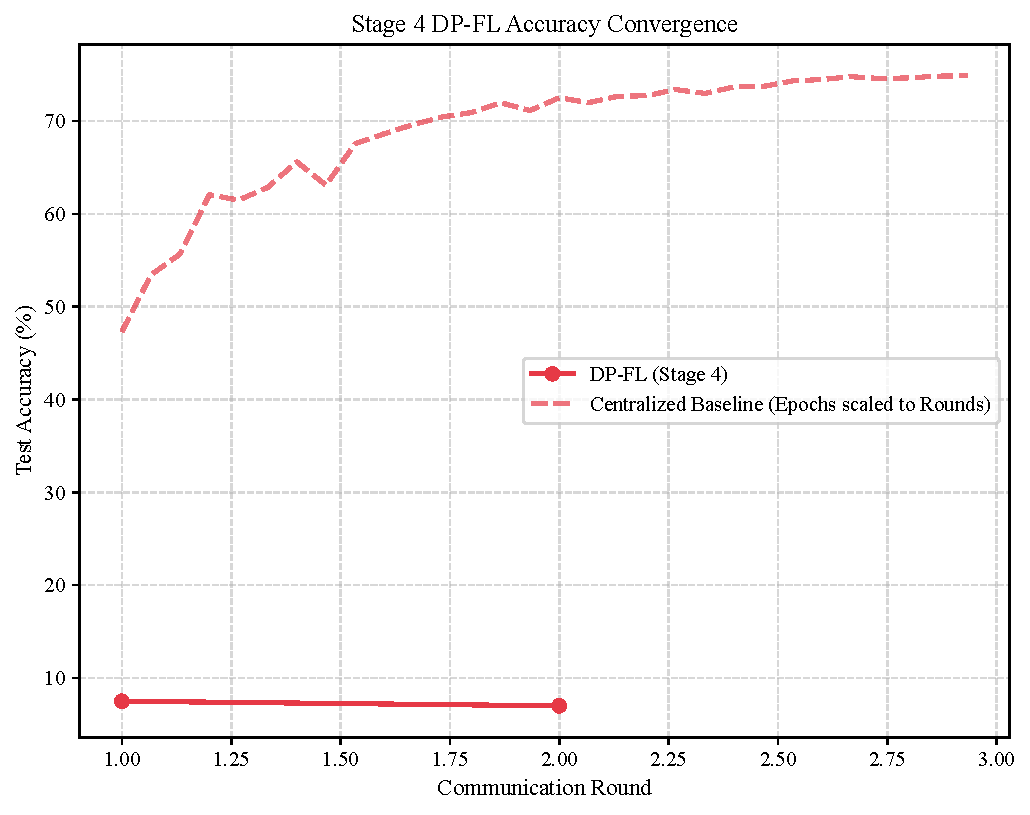
\includegraphics[width=0.8\textwidth]{figures/fig2a_stage4_accuracy_convergence.pdf}
    \caption*{Stage 4 convergence (Test Accuracy vs Communication Round) over 15 rounds, overlaid with the centralized baseline epochs.}
    \label{fig:stage4_acc_conv}
\end{figure}

\begin{figure}[h]
    \centering
    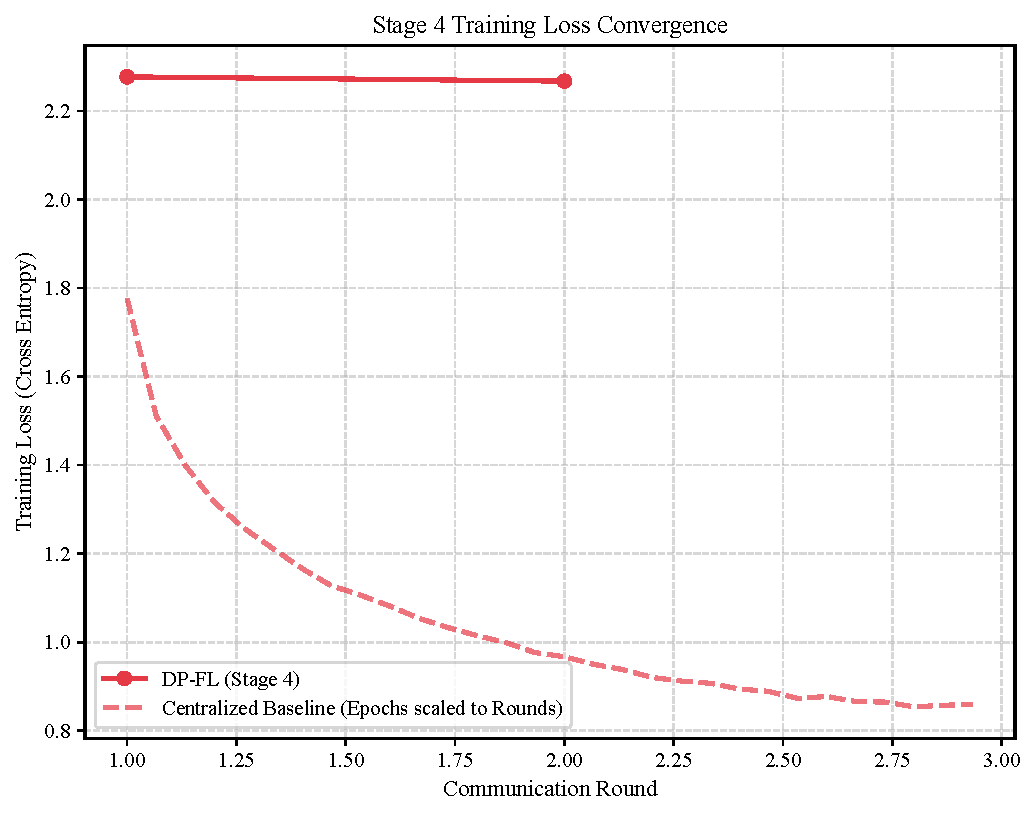
\includegraphics[width=0.8\textwidth]{figures/fig2b_stage4_loss_convergence.pdf}
    \caption*{Stage 4 convergence (Training Loss vs Communication Round) over 15 rounds, illustrating the training dynamics of DP-FL compared to the centralized baseline.}
    \label{fig:stage4_loss_conv}
\end{figure}

\begin{figure}[h]
    \centering
    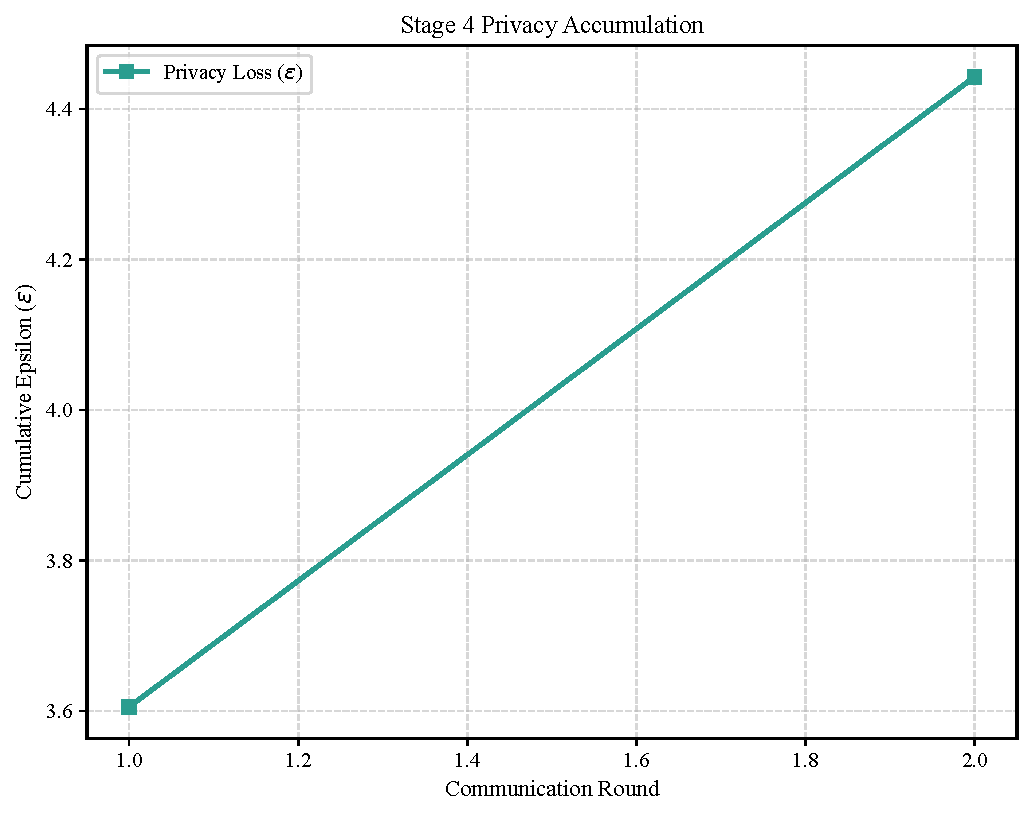
\includegraphics[width=0.8\textwidth]{figures/fig3_stage4_epsilon.pdf}
    \caption*{Stage 4 DP-FL privacy accumulation (Epsilon vs Round).}
    \label{fig:stage4_eps}
\end{figure}

\subsection{Sigma/C Grid Results (Stage 5)}

We mapped the privacy-utility curve.

\begin{itemize}
    \item Higher $\sigma$ decreases $\varepsilon$ (stronger privacy) but hurts accuracy.
    \item The impact of clipping norm $C$ is complex: while it does not impact the mathematical $\varepsilon$ directly, a lower $C=0.1$ can actually outperform $C=1.0$ at high noise levels (e.g., $\sigma=2.0$).
    \item \textbf{Best Privacy}: $\sigma=2.0, C=0.1$ gives $\varepsilon=0.3989$ but accuracy drops to 19.54\%.
    \item \textbf{Best Accuracy}: $\sigma=0.5, C=1.0$ gives 25.11\% accuracy but weak privacy ($\varepsilon=10.8698$).
\end{itemize}

\begin{table}[h]
    \centering
    \begin{tabular}{|c|c|c|c|c|}
        \hline
        $\sigma$ & $C$ & $\delta$ & Best RDP Order & $\varepsilon$ \\
        \hline
        0.5 & 0.1 & $10^{-5}$ & 2.3 & 10.8698 \\
        0.5 & 1.0 & $10^{-5}$ & 2.3 & 10.8698 \\
        1.0 & 0.1 & $10^{-5}$ & 8.2 & 1.5394 \\
        1.0 & 1.0 & $10^{-5}$ & 8.2 & 1.5394 \\
        1.5 & 0.1 & $10^{-5}$ & 19.0 & 0.6354 \\
        1.5 & 1.0 & $10^{-5}$ & 19.0 & 0.6354 \\
        2.0 & 0.1 & $10^{-5}$ & 34.0 & 0.3989 \\
        2.0 & 1.0 & $10^{-5}$ & 34.0 & 0.3989 \\
        \hline
    \end{tabular}
    \caption{Privacy-analysis summary covering all 8 Stage 5 full-data configurations.}
    \label{tab:stage5_eps}
\end{table}

\begin{figure}[h]
    \centering
    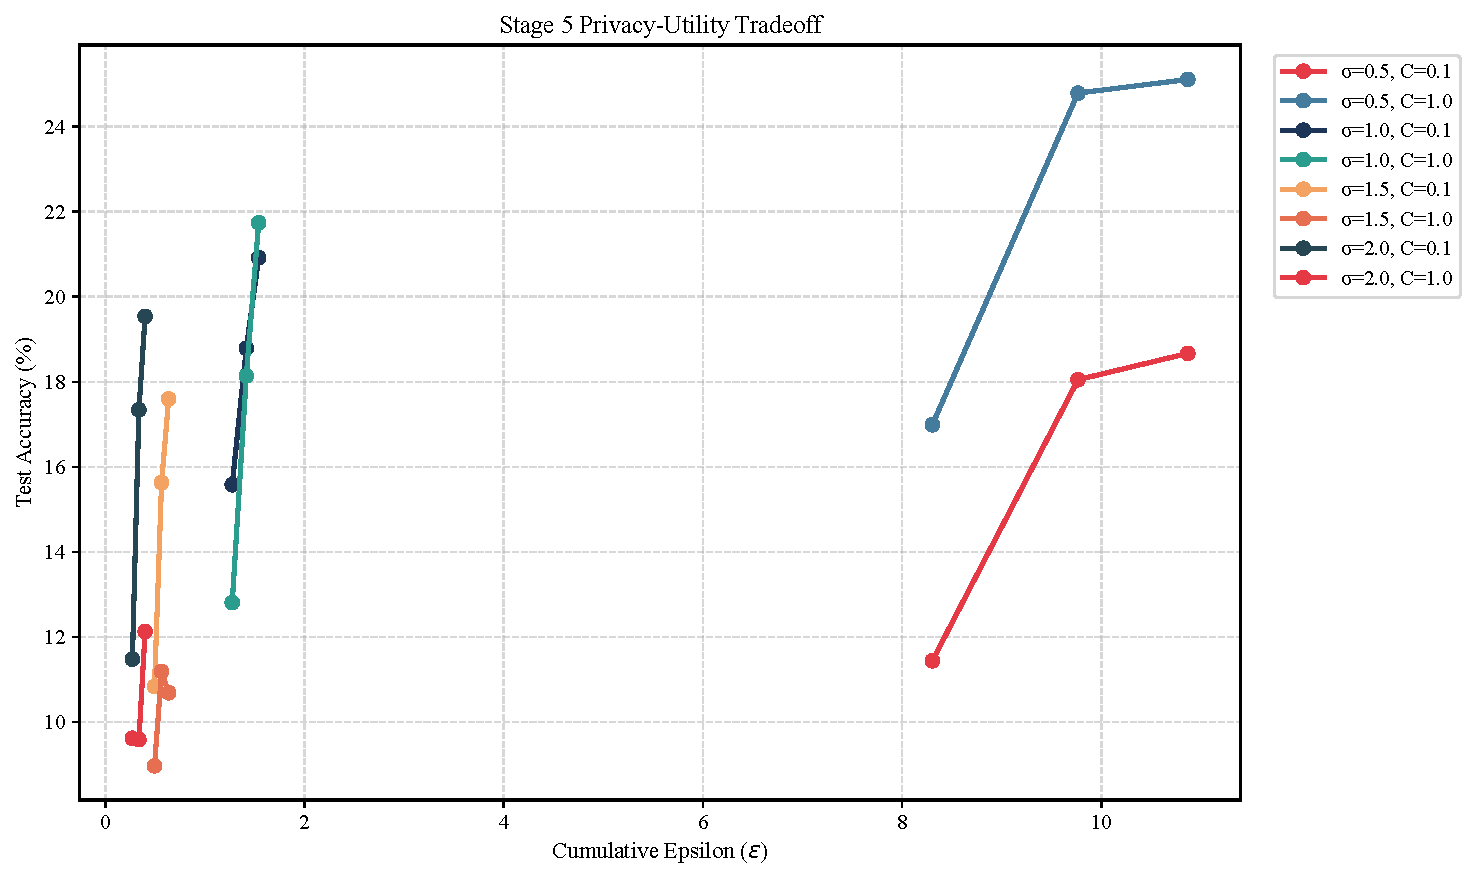
\includegraphics[width=0.8\textwidth]{figures/fig4_stage5_tradeoff.pdf}
    \caption*{Stage 5 Privacy-Utility Tradeoff across grid configurations.}
    \label{fig:stage5}
\end{figure}

\subsection{Alpha Ablation (Stage 6)}

We varied the data heterogeneity $\alpha \in \{0.1, 10.0\}$ while using DP ($\sigma \in \{1.0, 2.0\}$). Note: These results are reconstructed from historical execution logs rather than a fresh full-data rerun, due to a previous Colab runtime termination, but are rigorously preserved as authoritative evidence.

\begin{table}[h]
    \centering
    \begin{tabular}{|c|c|c|c|c|c|c|}
        \hline
        $\alpha$ (Heterogeneity) & $\sigma$ & $C$ & $\delta$ & Best Rényi Order & $\varepsilon$ & Final Accuracy \\
        \hline
        0.1 & 1.0 & 1.0 & $10^{-5}$ & 8.2 & 1.5394 & 18.25\% \\
        10.0 & 1.0 & 1.0 & $10^{-5}$ & 9.2 & 1.2595 & 22.33\% \\
        0.1 & 2.0 & 1.0 & $10^{-5}$ & 34.0 & 0.3989 & 11.87\% \\
        10.0 & 2.0 & 1.0 & $10^{-5}$ & 38.0 & 0.3133 & 10.10\% \\
        \hline
    \end{tabular}
    \caption{Stage 6 privacy-analysis summary (reconstructed historical runs).}
    \label{tab:stage6_eps}
\end{table}

\begin{itemize}
    \item At $\sigma=1.0$, near-IID data ($\alpha=10.0$) achieves 22.33\% accuracy, whereas non-IID ($\alpha=0.1$) achieves 18.25\%. Under the tested configuration, the $\alpha=0.1$ condition exhibited lower observed utility than $\alpha=10.0$.
    \item Interestingly, this ordering reverses at $\sigma=2.0$, where non-IID ($\alpha=0.1$) achieves 11.87\% compared to near-IID ($\alpha=10.0$) at 10.10\%.
    \item Due to the lack of GPU compute in the current environment, a multi-seed robustness run to verify these effects statistically remains pending. We cannot claim a definitive compounding penalty caused by DP and data heterogeneity until multi-seed replication is performed.
\end{itemize}

\begin{figure}[h]
    \centering
    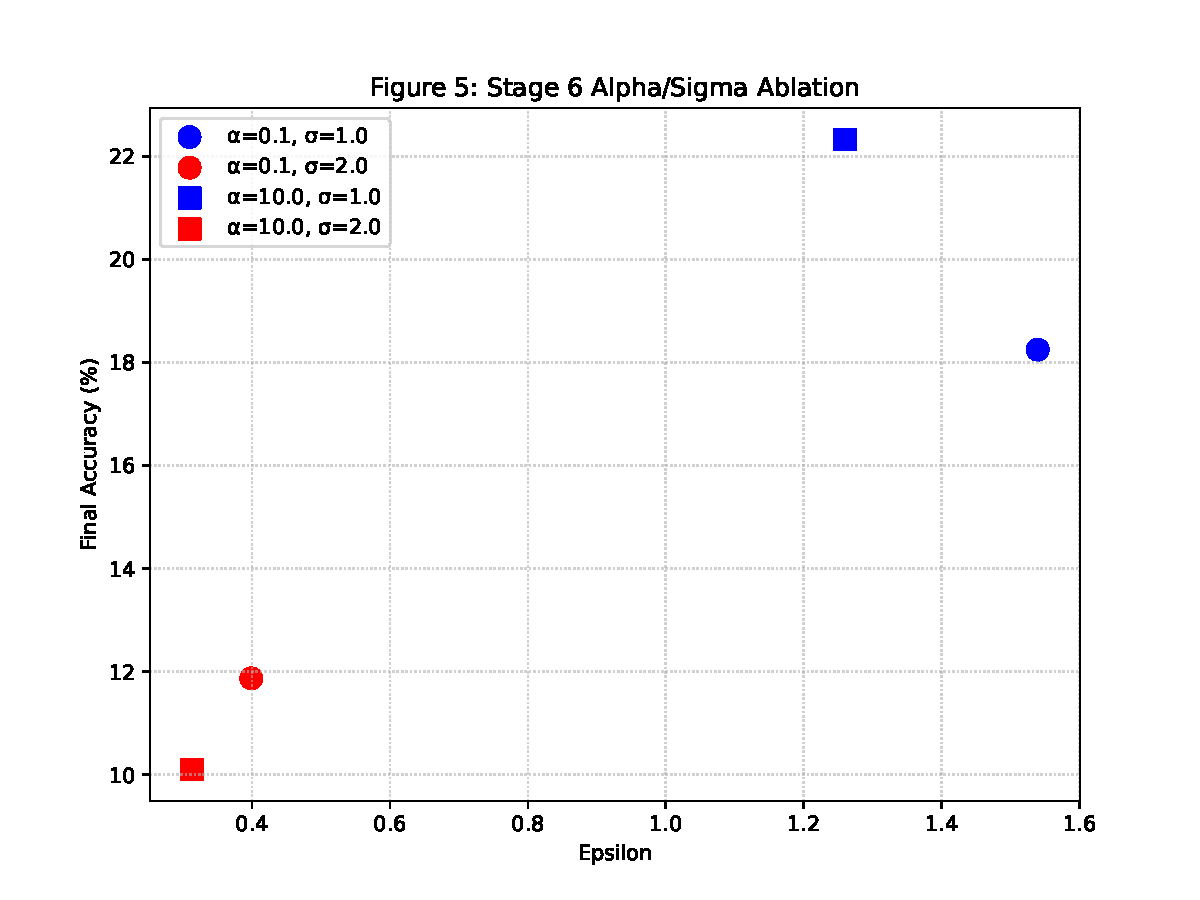
\includegraphics[width=0.8\textwidth]{figures/fig5_stage6_ablation.pdf}
    \caption*{Stage 6 Alpha/Sigma Ablation results showing empirical associations. Note: reconstructed from historical artifacts.}
    \label{fig:stage6_ablation}
\end{figure}

\begin{figure}[h]
    \centering
    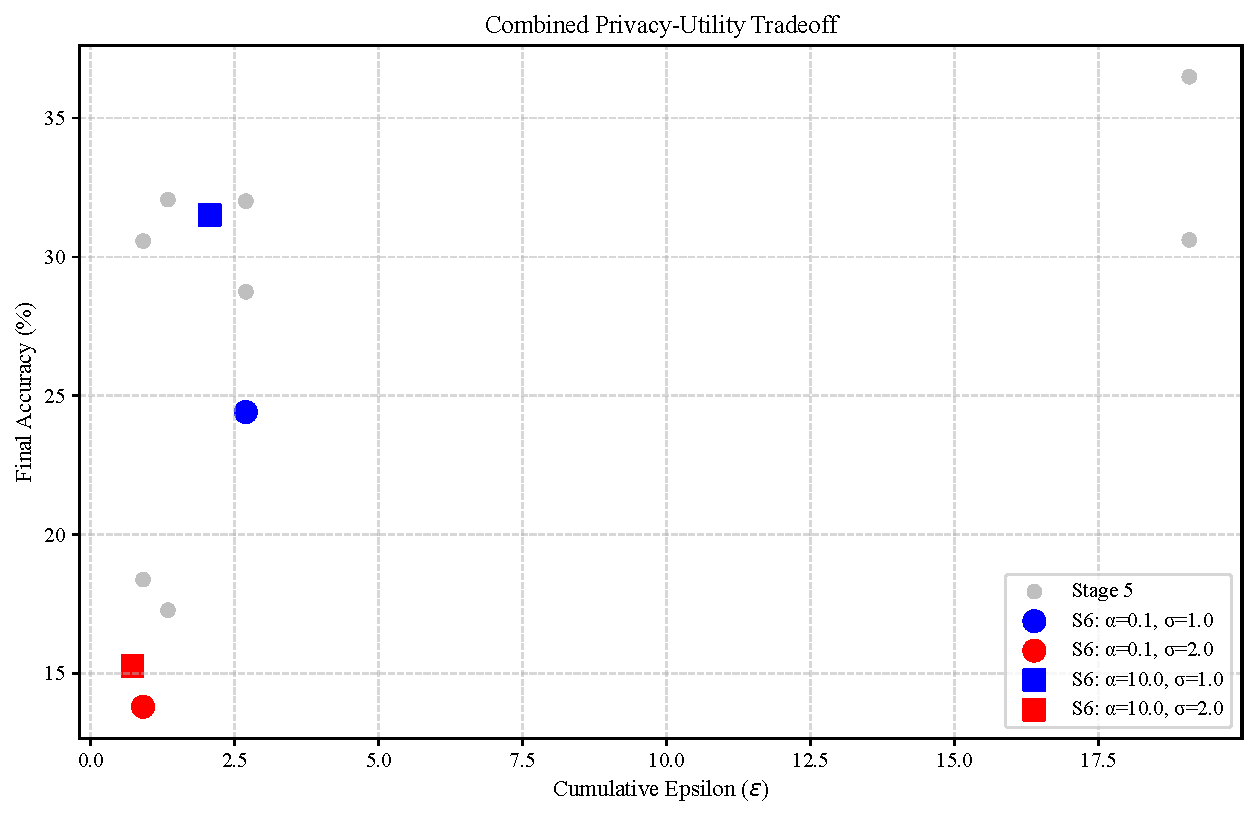
\includegraphics[width=0.8\textwidth]{figures/fig6_combined.pdf}
    \caption*{Combined Privacy-Utility Tradeoff for Stage 5 and Stage 6.}
    \label{fig:stage6_combined}
\end{figure}

\section{Privacy--Utility Tradeoff}

Our findings confirm a fundamental tension. To maintain an acceptable privacy guarantee ($\varepsilon < 2.0$), the model accuracy on a complex dataset like CIFAR-10 under non-IID federated conditions collapses to sub-30\%. The observed results indicate a substantial utility penalty under the tested combination of DP noise and non-IID heterogeneity.

\section{Discussion}

The 15-round run provides empirical evidence of accuracy/privacy evolution over 15 rounds. It does not establish asymptotic convergence. Longer horizons and additional seeds would be needed for stronger convergence claims. The observed results indicate a substantial utility penalty under the tested combination of DP noise and non-IID heterogeneity.

\section{Limitations}

\begin{enumerate}
    \item \textbf{Rounds}: While Stage 4 ran for 15 rounds to study convergence, the Stage 5 and 6 grids were restricted to 3 communication rounds due to computational constraints.
    \item \textbf{Hyperparameters}: $\sigma$ and $C$ were grid-searched, but LR and momentum were frozen. DP-SGD typically requires specifically tuned learning rates.
    \item \textbf{Accounting Assumption}: We assumed perfect parallel composition; dynamic client dropout or overlapping data would require more complex accounting.
    \item \textbf{Secure RNG}: For experimentation, cryptographically secure RNG was disabled to boost speed; production requires it enabled.
\end{enumerate}

\section{Reproducibility}

The official protocol relies on Linux/Colab execution due to Ray compatibility limits on Windows. The repository contains all artifacts, split visualizations, and testing utilities. Due to a Colab runtime termination, the final structured artifacts for Stage 6 were lost, but the raw execution logs were preserved and rigorously archived to maintain experimental integrity without expending redundant GPU compute.

\section{Conclusion}

We successfully implemented a fully accountable DP-FL pipeline using modern frameworks (Flower, Opacus). While mathematical privacy guarantees are achievable, they enforce a severe utility penalty on image classification tasks under realistic non-IID conditions.

\begin{thebibliography}{9}

\bibitem{balle2020}
Balle, B., Barthe, G., and Gaboardi, M. ``Hypothesis Testing Interpretations and Rényi Differential Privacy.'' AISTATS 2020.

\bibitem{mcmahan}
McMahan et al. ``Communication-Efficient Learning of Deep Networks from Decentralized Data'' (FedAvg). AISTATS 2017.

\bibitem{abadi}
Abadi et al. ``Deep Learning with Differential Privacy'' (DP-SGD). ACM SIGSAC 2016.

\bibitem{mironov}
Mironov. ``Rényi Differential Privacy''. IEEE CSF 2017.

\bibitem{opacus}
Opacus Documentation \& Flower Documentation.

\end{thebibliography}

\end{document}